\section{AVL Tree}

AVL tree is a height balanced binary search tree. Every node stores a balance factor 
$$
BF(x) = \id{height}(\attrib{x}{left}) - \id{height}(\attrib{x}{right})
$$
To keep an AVL tree balanced, we need to maintain the invariant that every node in an AVL tree has balance factor of -1, 0, or 1.

AVL tree was invented by Adelson-Velski and Landis, and hence the name AVL tree.

\begin{theorem}
    The height of an AVL tree with $n$ nodes is $O(\log n)$.
\end{theorem}

\begin{proof}
    Let $M(h)$ be the minimum number of nodes in any AVL tree with height $h$. $M$ could be recursively defined such that $M(0)=1$, $M(1)=2$, and for all $h \geq 2$, $M(h) = 1 + M(h-1) + M(h-2)$.
    
    We can obtain a closed form of this recurrence, $M(h) = F_{h+3} - 1$ where $F_k$ represents the $k$th Fibonacci number. Because $F_h > \frac{\phi^h}{\sqrt{5}} - 1$ where $\phi = \frac{1+\sqrt{5}}{2}$ is the golden ratio,
    $$
    n \geq M(h) > \left( \frac{\phi^{h+3}}{\sqrt{5}} - 2 \right) 
    $$
    and
    $$
    h < 1.44 \log_2 (n+2)
    $$
\end{proof}

An alternative proof:

\begin{proof}
    $M(h) > M(h-1)$, so $M(h-1)>M(h-2)$ for all $h\geq 2$. It follows that
    $$
    M(h) = 1 + M(h-1) + M(h-2) > 2M(h-2)
    $$
    Substitute $h-2$ for $h$, and we get $M(h-2) > 2M(h-4)$. It can be shown using induction that $M(h) > 2^k M(h-2k)$ for $k>0$.

    Take $k = h/2$. Then, $M(h) > 2^{h/2} M(0) = 2^{h/2}$. Taking logarithm of both sides, we get $h < 2 \log_2 M(h)$, and thus $h \in O(n \log n)$.   
\end{proof}

\subsection{AVL Insertion}

At a high level, insertion to an AVL tree works as follows:
\begin{enumerate}
    \item Perform standard BST insertion.
    \item From the inserted node up to the root, update the balance factor, and perform rotations as necessary.
\end{enumerate}

For AVL insertion, we can prove that 1 rotation is sufficient to restore height balance of the entire tree. The idea of the proof is to look at the height of subtrees before the insertion, and compare with the height of the subtrees after the insertion.

\subsection{AVL Deletion}

At a high level, to delete a node from an AVL tree, we perform the following operations:

\begin{enumerate}
    \item Perform standard BST deletion
    \begin{itemize}
        \item If $x$ has no children, $x$ is a leaf and can be safely removed;
        \item If $x$ has one child $y$, then $y$ is a leaf. Replace $x$ with $y$ and remove $y$;
        \item $x$ has two children. Replace $x$ with its successor $y$. Remove $y$ by following one of the previous two cases
    \end{itemize}
    \item From deleted leaf up to the root, update the balance factor and perform rotations as necessary.
\end{enumerate}

\subsection{AVL Rotation Recipes}

If we detect a imbalance at a node $x$ where $|BF(x)| > 1$, perform the following checks and rotate accordingly

\begin{itemize}
    \item LL: $\id{height}(\attribb{x}{left}{left}) \geq \id{height}(\attribb{x}{left}{right})$ 
    \item LR: $\id{height}(\attribb{x}{left}{left}) < \id{height}(\attribb{x}{left}{right})$ 
    \item RR: $\id{height}(\attribb{x}{right}{right}) \geq \id{height}(\attribb{x}{right}{right})$ 
    \item RL: $\id{height}(\attribb{x}{right}{right}) < \id{height}(\attribb{x}{right}{left})$ 
\end{itemize}

\begin{figure}[htbp]
    \centering
    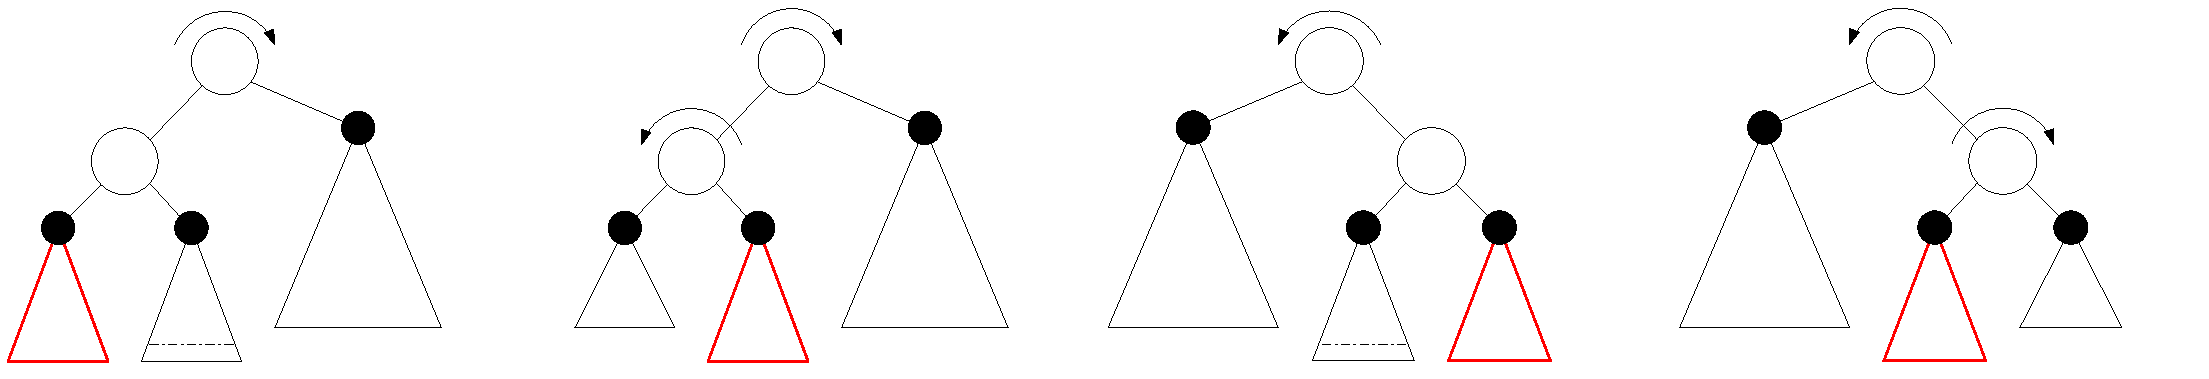
\includegraphics[width=\linewidth]{avl-rotation-recipes-oneline.pdf}
    \caption{AVL rotation recipes, from left to right: LL, LR, RR, RL cases}
    \label{fig:avl-rotation}
\end{figure}

In particular, after insertion, we only need one rotation to fix the imbalance. After deletion, as we retrace back to the root, we might need to fix multiple nodes along the path to root.